\documentclass{standalone}
\usepackage{pgfplots}
\pgfplotsset{compat=1.18}
\begin{document}
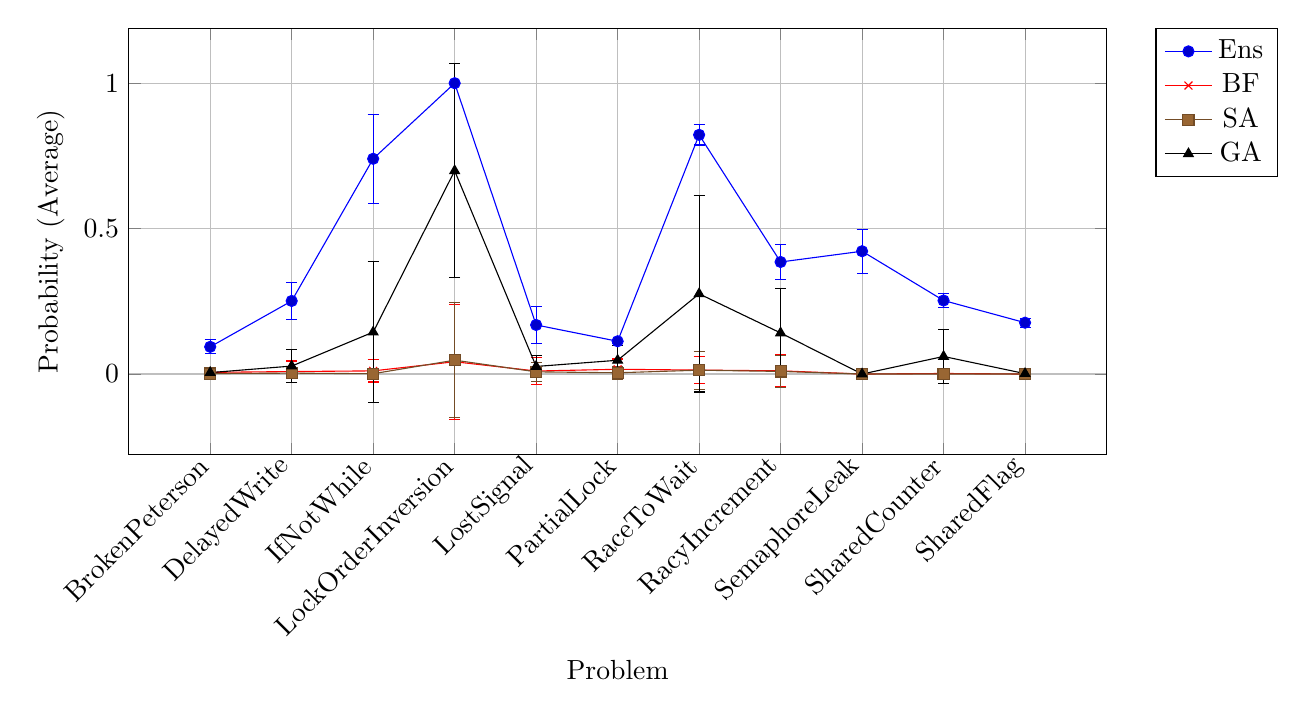
\begin{tikzpicture}
\begin{axis}[
    width=14cm, height=7cm,
    xlabel={Problem},
    ylabel={Probability (Average)},
    xtick=data,
    xticklabels={BrokenPeterson,DelayedWrite,IfNotWhile,LockOrderInversion,LostSignal,PartialLock,RaceToWait,RacyIncrement,SemaphoreLeak,SharedCounter,SharedFlag},
    xticklabel style={rotate=45, anchor=east},
    legend style={at={(1.05,1)}, anchor=north west},
    grid=both,
    error bars/y dir=both,
    error bars/y explicit
]
\addplot+[mark=*, error bars/.cd, y dir=both, y explicit] coordinates { (0,0.09358000000000001) +- (0,0.02435627564438588) (1,0.2512400000000001) +- (0,0.0646695083182362) (2,0.7401599999999999) +- (0,0.1529480850965248) (3,1.0) +- (0,0.0) (4,0.16874) +- (0,0.06339439555477373) (5,0.11266) +- (0,0.005836584128213547) (6,0.8224000000000001) +- (0,0.03505272995860693) (7,0.3852799999999999) +- (0,0.05935505067655488) (8,0.42225999999999997) +- (0,0.07566408308694297) (9,0.25283999999999995) +- (0,0.025212047654618923) (10,0.17656000000000002) +- (0,0.01580513995444494) };
\addlegendentry{Ens}
\addplot+[mark=x, error bars/.cd, y dir=both, y explicit] coordinates { (0,0.00578) +- (0,0.017645361302909165) (1,0.008539999999999999) +- (0,0.03643961177238925) (2,0.010860000000000002) +- (0,0.038050991566366224) (3,0.042260000000000006) +- (0,0.19792132120556166) (4,0.01034) +- (0,0.04537715419072663) (5,0.01636) +- (0,0.03553713780350502) (6,0.013600000000000001) +- (0,0.04670882449510248) (7,0.01098) +- (0,0.05437867604275838) (8,0.0) +- (0,0.0) (9,0.0018999999999999998) +- (0,0.007211810041982016) (10,0.0) +- (0,0.0) };
\addlegendentry{BF}
\addplot+[mark=square*, error bars/.cd, y dir=both, y explicit] coordinates { (0,0.00168) +- (0,0.011022129873067886) (1,0.0031) +- (0,0.01774910173064817) (2,0.00106) +- (0,0.005246612123600352) (3,0.04769999999999999) +- (0,0.196819636692468) (4,0.007540000000000002) +- (0,0.03217567213829449) (5,0.00434) +- (0,0.021483368032988132) (6,0.01322) +- (0,0.06554054361342189) (7,0.00902) +- (0,0.056137037139267605) (8,0.0) +- (0,0.0) (9,0.00012) +- (0,0.000848528137423857) (10,0.0) +- (0,0.0) };
\addlegendentry{SA}
\addplot+[mark=triangle*, error bars/.cd, y dir=both, y explicit] coordinates { (0,0.004940000000000001) +- (0,0.013418552493484837) (1,0.02737999999999999) +- (0,0.05780434628105046) (2,0.1441) +- (0,0.2429957797567518) (3,0.6988) +- (0,0.3679851372331357) (4,0.02605999999999999) +- (0,0.037282928193663634) (5,0.04738000000000001) +- (0,0.050279581606558855) (6,0.27577999999999997) +- (0,0.3375984990052715) (7,0.14128) +- (0,0.15162440706009883) (8,4e-05) +- (0,0.000282842712474619) (9,0.060439999999999994) +- (0,0.09386467897555328) (10,0.0014000000000000002) +- (0,0.009899494936611667) };
\addlegendentry{GA}
\end{axis}
\end{tikzpicture}
\end{document}